\documentclass{standalone}
\usepackage{tikz}
\usetikzlibrary{patterns, positioning}
\usepackage[sfdefault]{ClearSans} %% option 'sfdefault' activates Clear Sans as the default text font
\usepackage[T1]{fontenc}

\begin{document}
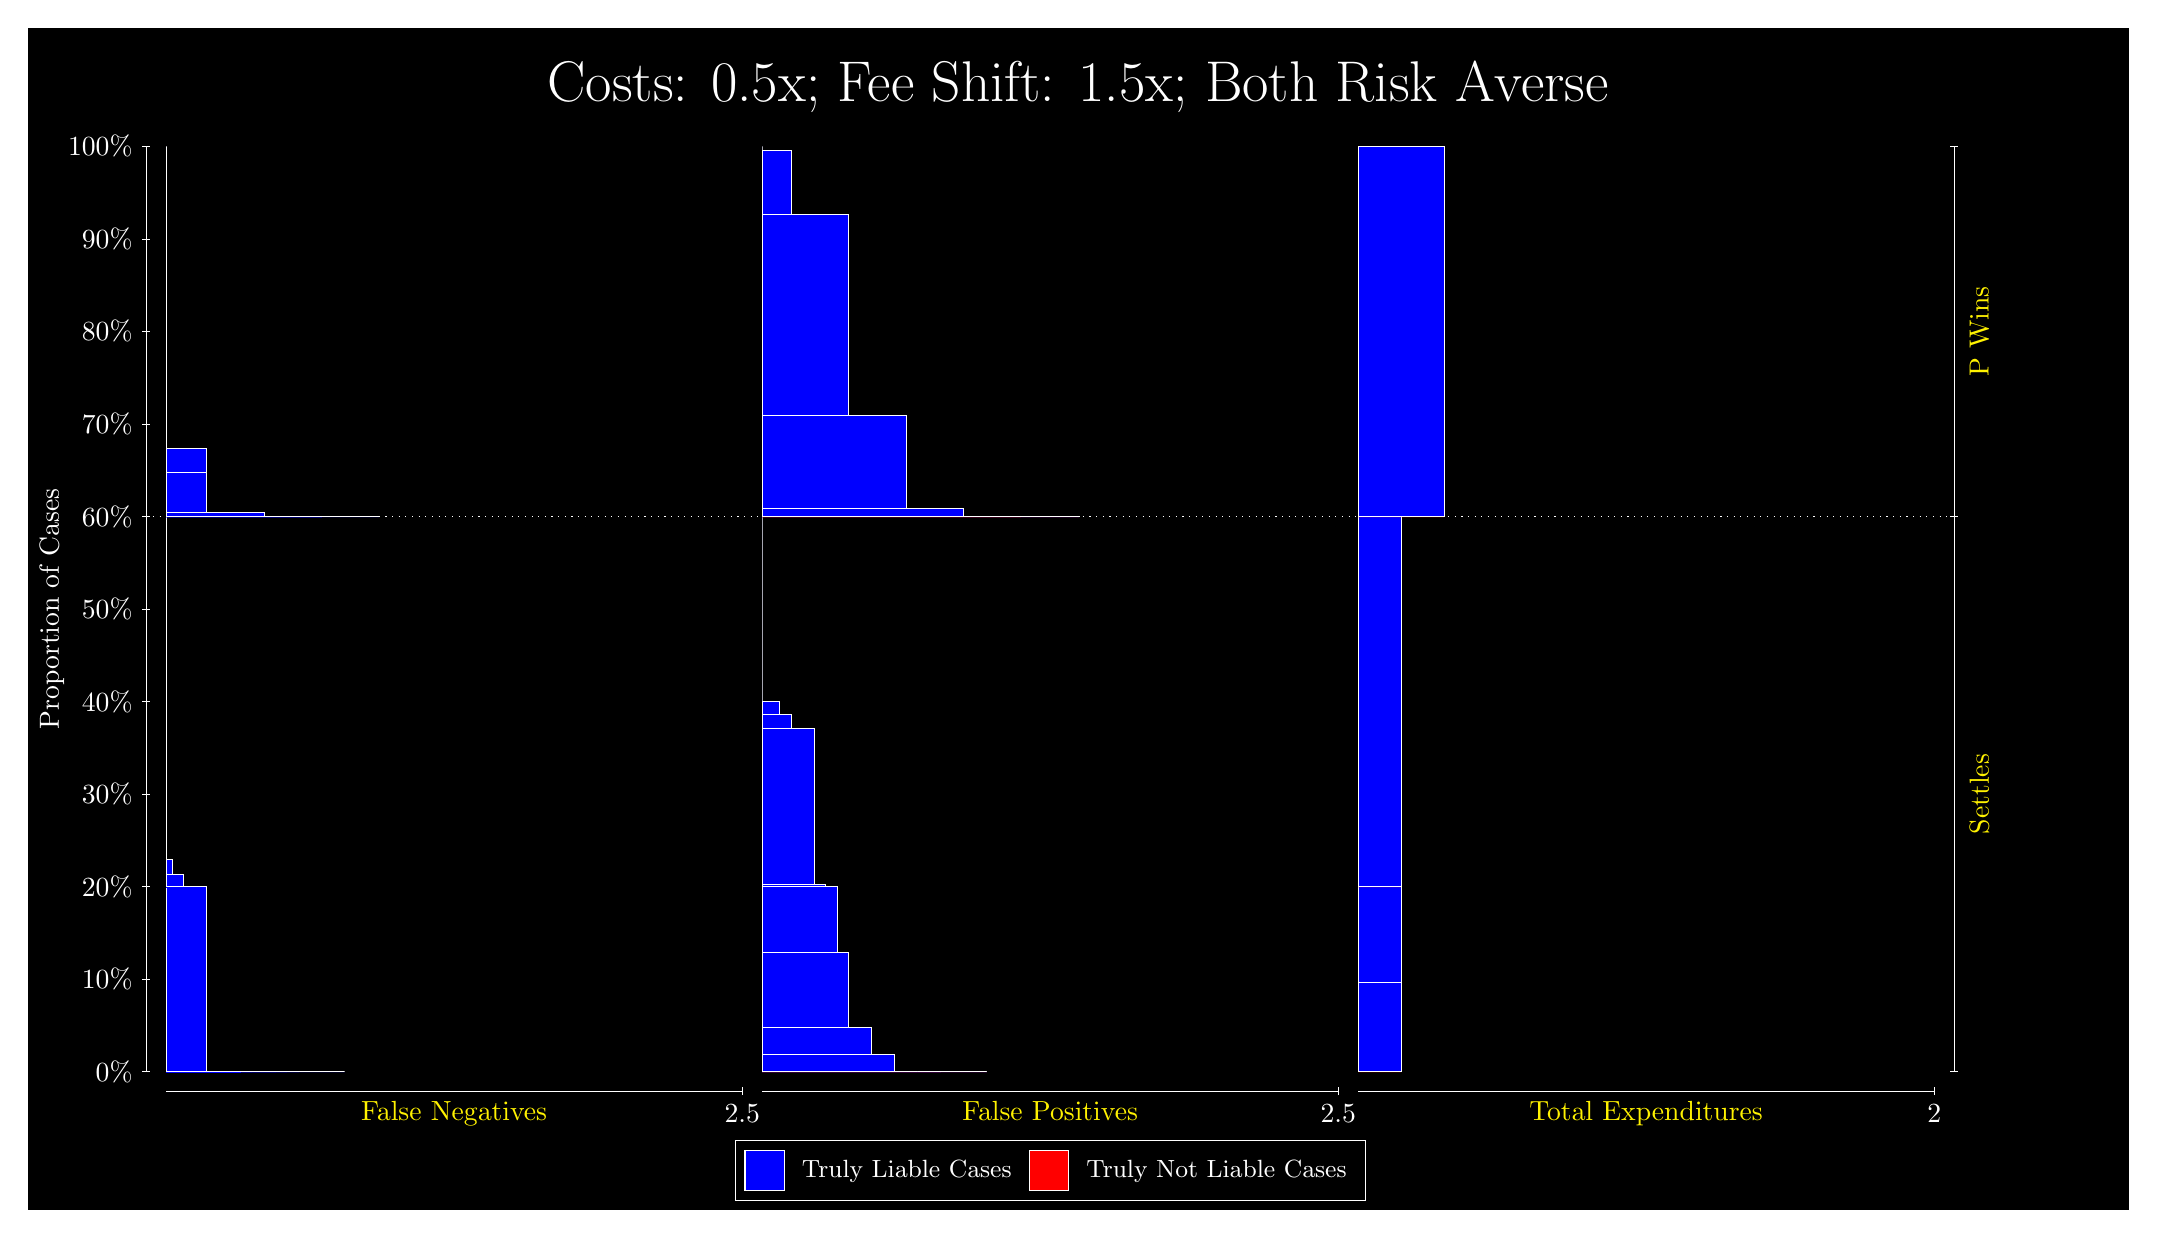
\begin{tikzpicture}
\draw[fill=black] (0,0) rectangle (26.667,15);
\draw[text=white] (0,13.5) rectangle (26.667,15) node[midway] {\huge Costs: 0.5x; Fee Shift: 1.5x; Both Risk Averse};
\draw[white, very thin] (1.5,1.75) -- (1.5,13.5);
\node[rotate=90, text=white, anchor=center] at (0.3, 7.625) {Proportion of Cases};
\draw[white, very thin] (1.45,1.75) -- (1.55,1.75);
\node[text=white, anchor=east] at (1.45, 1.75) {0\%};
\draw[white, very thin] (1.45,2.925) -- (1.55,2.925);
\node[text=white, anchor=east] at (1.45, 2.925) {10\%};
\draw[white, very thin] (1.45,4.1) -- (1.55,4.1);
\node[text=white, anchor=east] at (1.45, 4.1) {20\%};
\draw[white, very thin] (1.45,5.275) -- (1.55,5.275);
\node[text=white, anchor=east] at (1.45, 5.275) {30\%};
\draw[white, very thin] (1.45,6.45) -- (1.55,6.45);
\node[text=white, anchor=east] at (1.45, 6.45) {40\%};
\draw[white, very thin] (1.45,7.625) -- (1.55,7.625);
\node[text=white, anchor=east] at (1.45, 7.625) {50\%};
\draw[white, very thin] (1.45,8.8) -- (1.55,8.8);
\node[text=white, anchor=east] at (1.45, 8.8) {60\%};
\draw[white, very thin] (1.45,9.975) -- (1.55,9.975);
\node[text=white, anchor=east] at (1.45, 9.975) {70\%};
\draw[white, very thin] (1.45,11.15) -- (1.55,11.15);
\node[text=white, anchor=east] at (1.45, 11.15) {80\%};
\draw[white, very thin] (1.45,12.325) -- (1.55,12.325);
\node[text=white, anchor=east] at (1.45, 12.325) {90\%};
\draw[white, very thin] (1.45,13.5) -- (1.55,13.5);
\node[text=white, anchor=east] at (1.45, 13.5) {100\%};

\draw[white, very thin] (24.457,1.75) -- (24.457,13.5);
\draw[white, very thin] (24.407,1.75) -- (24.507,1.75);
\node[anchor=west] at (24.407, 1.75) {};
\draw[white, very thin] (24.407,8.7978) -- (24.507,8.7978);
\node[anchor=west] at (24.407, 8.7978) {};
\draw[white, very thin] (24.407,13.5) -- (24.507,13.5);
\node[anchor=west] at (24.407, 13.5) {};

\draw[white, very thin, fill=blue] (1.75,1.75) rectangle (4.0188,1.75);
\draw[white, very thin, fill=blue] (1.75,1.75) rectangle (3.4333,1.75);
\draw[white, very thin, fill=blue] (1.75,1.75) rectangle (3.287,1.75);
\draw[white, very thin, fill=blue] (1.75,1.75) rectangle (3.1406,1.75);
\draw[white, very thin, fill=blue] (1.75,1.75) rectangle (2.8478,1.75);
\draw[white, very thin, fill=blue] (1.75,1.75) rectangle (2.7015,1.7503);
\draw[white, very thin, fill=blue] (1.75,1.7503) rectangle (2.5551,1.7516);
\draw[white, very thin, fill=blue] (1.75,1.7516) rectangle (2.4087,1.7516);
\draw[white, very thin, fill=blue] (1.75,1.7516) rectangle (2.2623,4.0977);
\draw[white, very thin, fill=blue] (1.75,4.0977) rectangle (2.1159,4.0991);
\draw[white, very thin, fill=blue] (1.75,4.0991) rectangle (1.9696,4.2557);
\draw[white, very thin, fill=blue] (1.75,4.2557) rectangle (1.8232,4.4405);
\draw[white, very thin, fill=red] (1.75,4.4405) rectangle (1.75,4.4405);
\draw[white, very thin, fill=blue] (1.75,4.4405) rectangle (1.75,8.7978);
\draw[white, very thin, fill=blue] (1.75,8.7978) rectangle (4.458,8.7978);
\draw[white, very thin, fill=blue] (1.75,8.7978) rectangle (3.7261,8.798);
\draw[white, very thin, fill=blue] (1.75,8.798) rectangle (2.9942,8.8473);
\draw[white, very thin, fill=blue] (1.75,8.8473) rectangle (2.2623,9.3545);
\draw[white, very thin, fill=blue] (1.75,9.3545) rectangle (2.2623,9.6673);
\draw[white, very thin, fill=red] (1.75,9.6673) rectangle (1.75,9.6673);
\draw[white, very thin, fill=blue] (1.75,9.6673) rectangle (1.75,13.5);
\draw[white, very thin, fill=red] (9.3189,1.75) rectangle (12.173,1.75);
\draw[white, very thin, fill=blue] (9.3189,1.75) rectangle (12.173,1.75);
\draw[white, very thin, fill=red] (9.3189,1.75) rectangle (11.588,1.75);
\draw[white, very thin, fill=blue] (9.3189,1.75) rectangle (11.588,1.75);
\draw[white, very thin, fill=blue] (9.3189,1.75) rectangle (11.441,1.7516);
\draw[white, very thin, fill=red] (9.3189,1.7516) rectangle (11.295,1.7516);
\draw[white, very thin, fill=blue] (9.3189,1.7516) rectangle (11.295,1.7516);
\draw[white, very thin, fill=red] (9.3189,1.7516) rectangle (11.002,1.7516);
\draw[white, very thin, fill=blue] (9.3189,1.7516) rectangle (11.002,1.9728);
\draw[white, very thin, fill=blue] (9.3189,1.9728) rectangle (10.856,1.9741);
\draw[white, very thin, fill=blue] (9.3189,1.9741) rectangle (10.709,2.3172);
\draw[white, very thin, fill=blue] (9.3189,2.3172) rectangle (10.563,2.3174);
\draw[white, very thin, fill=red] (9.3189,2.3174) rectangle (10.417,2.3174);
\draw[white, very thin, fill=blue] (9.3189,2.3174) rectangle (10.417,3.2708);
\draw[white, very thin, fill=blue] (9.3189,3.2708) rectangle (10.27,4.1022);
\draw[white, very thin, fill=blue] (9.3189,4.1022) rectangle (10.124,4.1317);
\draw[white, very thin, fill=blue] (9.3189,4.1317) rectangle (9.9776,6.1071);
\draw[white, very thin, fill=blue] (9.3189,6.1071) rectangle (9.8312,6.1073);
\draw[white, very thin, fill=blue] (9.3189,6.1073) rectangle (9.6848,6.2922);
\draw[white, very thin, fill=blue] (9.3189,6.2922) rectangle (9.5384,6.4488);
\draw[white, very thin, fill=blue] (9.3189,6.4488) rectangle (9.3921,6.4501);
\draw[white, very thin, fill=blue] (9.3189,6.4501) rectangle (9.3189,8.7978);
\draw[white, very thin, fill=red] (9.3189,8.7978) rectangle (13.344,8.7978);
\draw[white, very thin, fill=blue] (9.3189,8.7978) rectangle (13.344,8.7979);
\draw[white, very thin, fill=red] (9.3189,8.7979) rectangle (12.612,8.7979);
\draw[white, very thin, fill=blue] (9.3189,8.7979) rectangle (12.612,8.7991);
\draw[white, very thin, fill=red] (9.3189,8.7991) rectangle (11.88,8.7991);
\draw[white, very thin, fill=blue] (9.3189,8.7991) rectangle (11.88,8.9052);
\draw[white, very thin, fill=red] (9.3189,8.9052) rectangle (11.149,8.9052);
\draw[white, very thin, fill=blue] (9.3189,8.9052) rectangle (11.149,10.085);
\draw[white, very thin, fill=red] (9.3189,10.085) rectangle (10.417,10.085);
\draw[white, very thin, fill=blue] (9.3189,10.085) rectangle (10.417,12.631);
\draw[white, very thin, fill=blue] (9.3189,12.631) rectangle (9.6848,13.451);
\draw[white, very thin, fill=blue] (9.3189,13.451) rectangle (9.3189,13.5);
\draw[white, very thin, fill=red] (16.888,1.75) rectangle (17.437,1.75);
\draw[white, very thin, fill=blue] (16.888,1.75) rectangle (17.437,2.8896);
\draw[white, very thin, fill=red] (16.888,2.8896) rectangle (17.437,2.8896);
\draw[white, very thin, fill=blue] (16.888,2.8896) rectangle (17.437,4.099);
\draw[white, very thin, fill=red] (16.888,4.099) rectangle (17.437,4.099);
\draw[white, very thin, fill=blue] (16.888,4.099) rectangle (17.437,8.7978);
\draw[white, very thin, fill=red] (16.888,8.7978) rectangle (17.986,8.7978);
\draw[white, very thin, fill=blue] (16.888,8.7978) rectangle (17.986,13.5);
\draw[white, dotted] (1.5,8.7978) -- (24.457,8.7978);
\draw[white, very thin] (1.75,1.5) -- (9.0689,1.5);
\node[text=yellow, anchor=north] at (5.4094, 1.5) {False Negatives};
\draw[white, very thin] (9.0689,1.45) -- (9.0689,1.55);
\node[text=white, anchor=north] at (9.0689, 1.45) {2.5};

\draw[white, very thin] (9.3189,1.5) -- (16.638,1.5);
\node[text=yellow, anchor=north] at (12.978, 1.5) {False Positives};
\draw[white, very thin] (16.638,1.45) -- (16.638,1.55);
\node[text=white, anchor=north] at (16.638, 1.45) {2.5};

\draw[white, very thin] (16.888,1.5) -- (24.207,1.5);
\node[text=yellow, anchor=north] at (20.547, 1.5) {Total Expenditures};
\draw[white, very thin] (24.207,1.45) -- (24.207,1.55);
\node[text=white, anchor=north] at (24.207, 1.45) {2};

\node[text=yellow, centered, rotate=90] at (24.777, 5.2739) {Settles};
\node[text=yellow, centered, rotate=90] at (24.777, 11.149) {P Wins};

\draw (12.978300999999998,1.5) node[draw=none] (baseCoordinate) {};
\begin{scope}[align=center]
        \matrix[scale=0.5, draw=white, below=0.5cm of baseCoordinate, nodes={draw}, column sep=0.1cm]{
            \node[rectangle, draw, minimum width=0.5cm, minimum height=0.5cm, fill=blue] {}; &
            \node[draw=none, font=\small, text=white] (B) {Truly Liable Cases}; &
            \node[rectangle, draw, minimum width=0.5cm, minimum height=0.5cm, fill=red] {}; &
            \node[draw=none, font=\small, text=white] (B) {Truly Not Liable Cases}; \\
            };
\end{scope}

\end{tikzpicture}
\end{document}